\documentclass[11pt]{article}

\usepackage[margin=0.72in]{geometry}
\usepackage{amsmath,amssymb}
\usepackage{array}
\usepackage{booktabs}
\usepackage{graphicx}
\usepackage{longtable}
\usepackage{tabularx}
\usepackage{xcolor}
\usepackage{hyperref}
\usepackage{microtype}

\hypersetup{colorlinks=true,linkcolor=blue!55!black,urlcolor=blue!55!black}
\emergencystretch=2em
\setlength{\tabcolsep}{4.5pt}
\renewcommand{\arraystretch}{1.14}
\newcommand{\RouteA}{\textsc{Route-A}}
\newcommand{\pL}{p_{\mathrm L}}
\newcommand{\supported}{\textcolor{green!40!black}{supported}}
\newcommand{\conditional}{\textcolor{orange!75!black}{conditional}}
\newcommand{\blocked}{\textcolor{red!65!black}{not established}}
\newcolumntype{Y}{>{\raggedright\arraybackslash}X}
\newcolumntype{L}[1]{>{\raggedright\arraybackslash}p{#1}}

\title{Contract-Centric, Regime-Aware Safe Adaptive Dual-Loop Decoding\\
for Approximate GKP Quantum Memories}
\author{}
\date{Evidence-synchronized note; snapshot through T6.7.2, 17 July 2026}

\begin{document}
\maketitle

\begin{abstract}
Approximate Gottesman--Kitaev--Preskill (GKP) quantum error correction must
decode analog modular syndromes while the effective displacement, measurement,
and control statistics drift.  Earlier work in this repository organized this
problem around a CNN-assisted slow loop and an FPGA-oriented affine fast loop.
That architecture produced reusable simulation, fixed-point, and learning
evidence, but it did not establish that a CNN simultaneously improves logical
error rate (LER), tail safety, and latency against strong matched baselines.

This note therefore reorganizes the same technical stack around an execution
contract rather than a learned winner.  Static and adaptive MAP decoders own
the LER decision; a causal regime posterior, event state machine, conservative
fallback, and versioned A/B parameter banks own tail-safety decisions; and a
fixed-point fast path owns deterministic source-to-action execution.  CNN,
teacher, and distilled-student modules remain replaceable extensions that can
populate the same bounded parameter surface only after matched promotion
gates.

The current untouched smooth-drift formal matrix contains 576 trajectories and
28,311,552 scored decisions per method.  Relative to the pilot-locked EWMA
baseline, \RouteA{} reduces aggregate LER by
$2.1687\times10^{-5}$ (paired 95\% interval
$[1.9003,2.4548]\times10^{-5}$), a 2.14\% relative reduction.  This result is
regime-specific: only periodic drift survives Holm correction, and \RouteA{}
has higher aggregate LER than both static joint MAP and Window MAP.  Its
static-to-oracle gap closure is negative.  The current evidence therefore
supports a locked-EWMA, periodic-qualified smooth advantage, not general
superiority.  Separately, the fast-path core has a six-cycle execution
contract, target-device post-route estimates above 39.7 MHz, and a
board-independent million-cycle CXXRTL qualification with zero visible-field
mismatch.  These are deterministic pre-board engineering results, not measured
FPGA latency or external speed records.  The separate abrupt/OOD matrix contains
888 trajectories and 43,646,976 scored decisions per method.  All registered
non-inferiority gates passed against locked EWMA, but five families were exactly
tied on the core contrasts and static MAP was markedly better under calibration
shift.  This supports bounded pass-through safety, not a tail-performance
advantage.  Integrated \RouteA{} RTL, external comparisons, and real-board
measurements remain open gates.
\end{abstract}

\tableofcontents

\section{Scope, argument, and evidence cutoff}

The one-sentence argument of this note is:

\begin{quote}
For repeated approximate-GKP quantum-memory correction, a contract-centric
dual loop can assign average LER, tail safety, and deterministic execution to
separately testable modules; current evidence supports a narrow smooth-drift
gain over a locked EWMA comparator, abrupt/OOD non-inferiority to that same
locked comparator, and strong pre-board execution properties, but it does not
support universal LER, tail-performance superiority, external-SOTA, or
real-board claims.
\end{quote}

The old task board and
\path{docs/paper_notes/CNN_FPGA_GKP_theory_note_draft.tex} remain the historical
source for the CNN+FPGA affine-calibration line.  The current claim state is
instead governed by \path{docs/new_task_board.md}.  This note preserves useful
old results as extension evidence without allowing them to override newer
matched-comparison failures.  The physical setting follows analog GKP syndrome
decoding \cite{gkp2001,grimsmo2021}; the adaptive-decoder motivation is aligned
with evidence that decoder calibration and prior mismatch affect logical
performance \cite{chen2022,sivak2024}.

\begin{table}[htbp]
\centering
\small
\caption{Evidence cutoff used in this note.  ``Done'' refers to the current
task artifacts, not to a final paper or deployed system.}
\label{tab:evidence-cutoff}
\begin{tabularx}{\textwidth}{@{}l l X@{}}
\toprule
Surface & Status at cutoff & Consequence for this note \\
\midrule
T6.5.1--T6.5.3 & Done & Claim roles, unified execution contract, and formal protocol are frozen. \\
T6.6.1--T6.6.3 & Done & Comparator runner and V4 Window/EWMA dual-shadow policy are frozen before formal access. \\
T6.7.1 & Done & Untouched smooth formal matrix may support only its registered contrasts and boundaries. \\
T6.7.2 & Done & Abrupt/OOD and nominal gates support locked-EWMA non-inferiority, not tail or static-MAP superiority. \\
T6.7.3 & In Progress & Integrated long-sequence fixed-point/RTL qualification remains open. \\
T6.7.4--T6.9 & Todo or hardware-blocked & Promotion, external comparison, integrated P\&R, and real-board claims remain closed. \\
\bottomrule
\end{tabularx}
\end{table}

\subsection{Terminology ledger}

The following names are used consistently throughout the note.

\begin{table}[htbp]
\centering
\small
\caption{Canonical terminology and authority boundaries.}
\label{tab:terminology}
\begin{tabularx}{\textwidth}{@{}L{0.22\textwidth} L{0.30\textwidth} Y@{}}
\toprule
Canonical term & Definition & What it does not mean \\
\midrule
\RouteA{} safe adaptive dual loop & Full contract-centric system: MAP experts, causal routing, event/fallback logic, A/B banks, and fast path & A synonym for the CNN, teacher, student, or oracle \\
Static joint MAP & Observed-only strong software comparator using a fixed noise model & Current phase-LUT RTL equivalence; that promotion is blocked \\
Window MAP / EWMA adaptive MAP & Observed-only adaptive MAP experts updated from completed causal windows & Hidden-state or per-scenario oracle tuning \\
Regime posterior & Causal HMM/event evidence used to route between validated expert banks & A direct logical correction or privileged truth channel \\
Tail-safety layer & Event FSM, health flags, fallback, leakage/reset handling, and integrity rollback & Tail-performance superiority; T6.7.2 establishes only locked-EWMA non-inferiority \\
Fast path & Quantized phase-LUT, event, frame, and bank action with a six-cycle contract & Measured end-to-end board latency \\
Learning extension & Legacy CNN, Feedback-GRAPE teacher, or distilled student behind the same contract & The required main-system winner \\
Hidden-state oracle & Nondeployable model reference evaluated in an isolated truth lane & A deployable comparator or a paper-level recovery optimum \\
\bottomrule
\end{tabularx}
\end{table}

\section{Why the architecture changed without discarding the old work}

The earlier CNN-centric line produced a useful design pattern: a slow estimator
updates a low-dimensional correction surface, while the latency-critical path
uses a small quantized rule.  It also produced a frozen four-scenario result in
which a teacher-anchored residual branch outperformed UKF.  However, later
evidence exposed three limitations.

First, the learned strong branch did not survive the unified evidence gate.
T5.1.4 found no matched learned decoder in the registered matrix, no Holm
discoveries across 24 family tests, and a calibration-shift transient in which
the adaptive candidate had 55 errors per 512 decisions against 37 for the
reference.  Second, a generic uncertainty fallback had a positive aggregate
OOD effect but significantly harmed the compound family and imposed a small
nominal cost.  Third, the first unified \RouteA{} integration run was much worse
than Window/EWMA because the policy froze or reverted the wrong state under
tail evidence.

These are not reasons to discard the affine fast path, the historical learned
results, or the hardware work.  They are reasons to change the unit of
contribution.  The new unit is an auditable contract that assigns each claim to
the module and evidence lane that can actually support it.

\section{Contract-centric dual-loop method}

\subsection{System overview and reuse of the dual-loop pipeline}

Figure~\ref{fig:dual-loop-architecture} is retained from the presentation
material because its interface structure survives the move away from a
CNN-centric claim.  The durable elements are observed syndrome history, a
bounded slow-loop proposal, safe publication of a complete parameter image,
versioned A/B banks, a quantized MAP-LUT, an event state machine, and a Pauli
frame update.  These interfaces, rather than the identity of one learned
estimator, define the reusable architecture.

\begin{figure}[htbp]
  \centering
  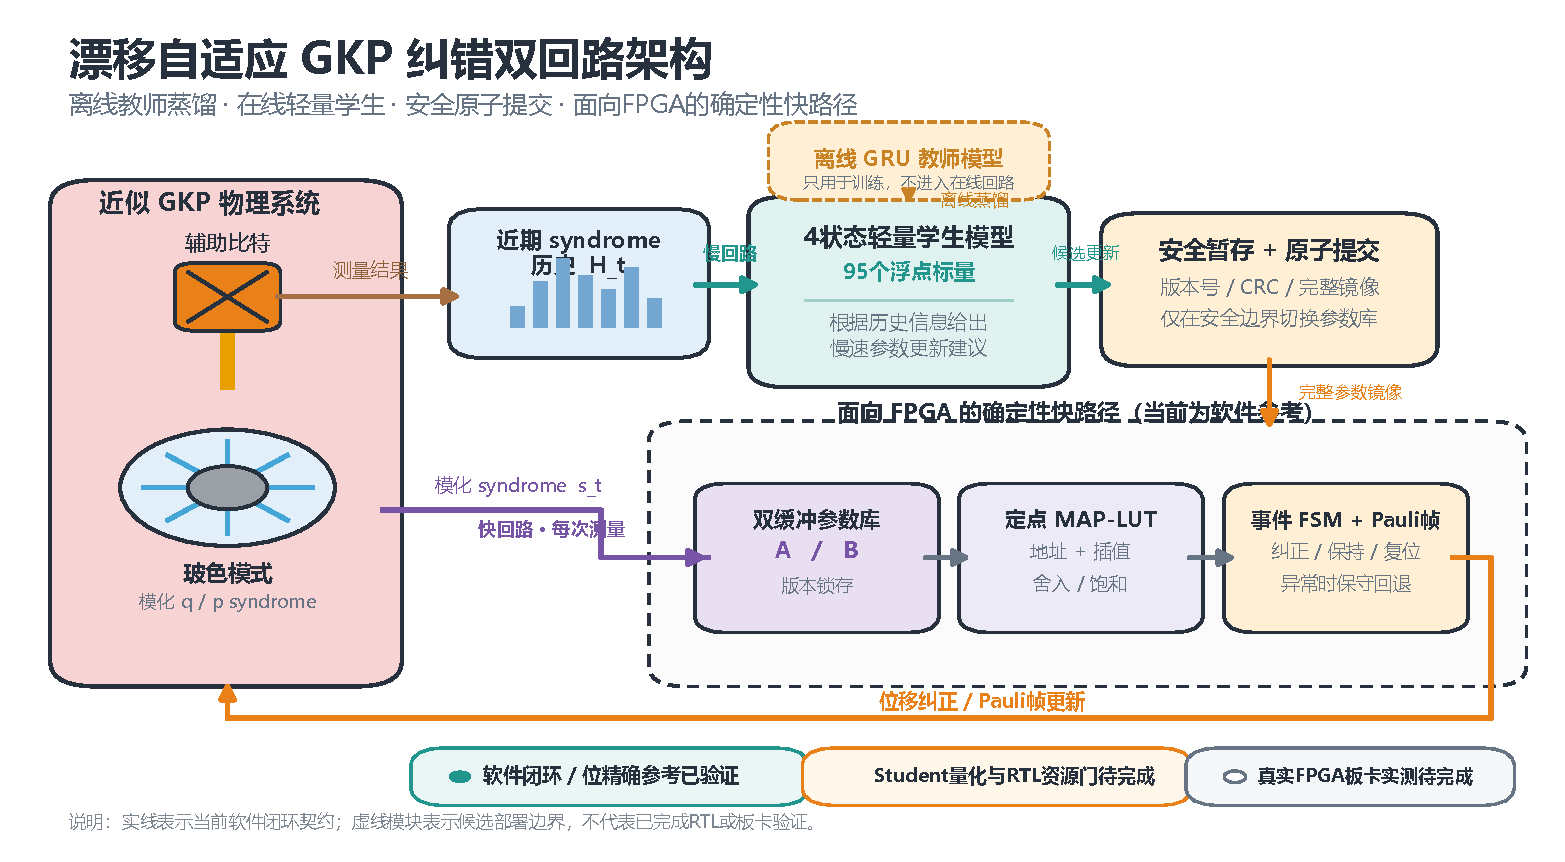
\includegraphics[width=\textwidth]{../figures/ppt_summary_20260716/drift_adaptive_architecture_cn.pdf}
  \caption{Reused Chinese presentation schematic of the drift-adaptive GKP
  dual loop.  Under the current \RouteA{} interpretation, the upper four-state
  student is an optional learning extension; Window and EWMA adaptive MAP
  provide the primary deployable parameter images, while HMM/event/fallback
  logic controls safe routing and publication.  The maturity badges in this
  16 July 2026 presentation asset are an archival snapshot: subsequent tasks
  added student fixed-point RTL and pre-board resource evidence, but real-board
  validation remains pending.}
  \label{fig:dual-loop-architecture}
\end{figure}

The fast loop consumes the current validated bank on every measurement and
never invokes the offline teacher.  The slow loop may host analytical,
filtering, or learned estimators, but each candidate must emit the same bounded
image and pass the same admission, integrity, and rollback rules.  The diagram
therefore acts as an interface map, not as evidence that the four-state student
is the main LER winner or that a complete FPGA deployment has been measured.

\subsection{Task formulation}

At cycle $t$, the deployable decoder receives only quantized observed syndrome
packets and health/event fields.  It returns a logical action, frame update,
fallback reason, active-bank identity, and versioned provenance.  Truth fields
used to generate trajectories are denied to all deployable adapters and are
available only to the isolated evaluator and model oracle.

For each completed parameter window, the host side maintains two causal expert
estimates:
\begin{equation}
  \widehat\theta_t^{\mathrm W}=\mathrm{Window}(y_{1:t}),
  \qquad
  \widehat\theta_t^{\mathrm E}=\mathrm{EWMA}(y_{1:t}),
\end{equation}
where $y_{1:t}$ denotes observed syndrome history only.  Each estimate compiles
to a parameter-bank image for the same fixed-point fast path.  The router may
promote the Window bank only when the causal smooth posterior, pre-update
predictive score, and hysteresis checks all pass.  Tail or uncertain evidence
uses the continuously updated and validated EWMA shadow; integrity faults alone
may republish the last-known-good image.

\subsection{Unified execution contract}

\begin{table}[htbp]
\centering
\small
\caption{Frozen execution fields shared by deployable methods.}
\label{tab:execution-contract}
\footnotesize
\begin{tabularx}{\textwidth}{@{}L{0.17\textwidth} L{0.27\textwidth} Y@{}}
\toprule
Field & Frozen value & Interpretation \\
\midrule
Syndrome quantization & 10-bit ADC; 8-bit LUT address; 2-bit fraction & Same quantized packet domain for every deployable comparator \\
MAP-LUT word & Signed Q9.12, ties-to-even, saturation & Deterministic arithmetic and packed-word behavior \\
Fast path & 5-cycle MAP plus 1-cycle event/action & Six-cycle logical action-valid contract \\
Bank protocol & CRC/SHA/CAS A/B bank, versioned commit, six-cycle drain & No silent partial publication; integrity-only LKG rollback \\
Cadence & 32-cycle regime update; 2,048 scalar samples; 4,000-cycle parameter update & Completed-window causality and explicit update age \\
Matched ceilings & 8,192 update MACs; 8,192 B state; 8,192 B workspace; 5,000 $\mu$s host update & Fail-fast budget admission, with actual use still reported \\
Oracle isolation & Separate exact-key truth packet & No deployable aggregate may consume hidden state \\
\bottomrule
\end{tabularx}
\end{table}

The current hardware LUT is phase-conditioned and is not mathematically
equivalent to the full two-dimensional joint MAP used as a strong software
comparator.  The latter is therefore retained in the comparison table but is
not relabelled as current-RTL deployable.

\subsection{Safety state and atomic updates}

The V4 policy replaced two failed architectures.  A static-switch design and a
freeze-all-EWMA design both failed all 38 pilot-safe candidate tuples because
the supposedly trusted state became stale under persistent calibration or
telegraph changes.  V4 instead updates Window and EWMA shadow banks
continuously.  A 20,061-cycle structural trace produced versions 1--4 at cycles
4001, 8002, 12003, and 16005; all source-to-action fields were six cycles.  At
the tail transition, the EWMA shadow was committed rather than reverting to
static.  An integrity fault cancelled a pending Window update and completed an
LKG rollback.  The registered dual-shadow update cost was 1,218 MACs under the
8,192-MAC ceiling.

This trace proves structural execution and provenance, not tail-performance
superiority.  The independent T6.7.2 matrix subsequently established bounded
non-inferiority to locked EWMA, as reported below.

\subsection{Replaceable learned modules}

Learning is outside the critical claim path.  A legacy CNN can propose a
bounded update, a non-Markovian teacher can supply an offline control target,
and a low-dimensional student can compress that target.  All three must obey
the same schema, cadence, bank, and failure rules.  In the unified runner, the
legacy CNN required 3,489,984 MACs, 1,586,368 B of state, and at least 65,536 B
of workspace, so it was correctly demoted to ablation-only under the frozen
budget.  This failure does not invalidate the contract; it demonstrates why
learned modules must be replaceable rather than definitional.

\section{Evaluation protocol and metrics}

\subsection{Result-blind formal design}

The formal protocol was frozen after disclosure of earlier counterexamples but
before access to the new formal split.  Calibration, pilot, and formal data use
12, 12, and 24 independent seed clusters.  The complete protocol contains 143
cells and 71,958,528 formal decisions per method across smooth and abrupt/OOD
families.  T6.7.1 consumed the smooth subset: four families, six held-out cells
per family, 24 formal clusters, and 576 trajectories.  T6.7.2 then consumed the
locked abrupt/OOD and nominal subset: six fault families, one nominal cell,
24 formal clusters, and 888 trajectories.  Together the two tasks exhaust the
pre-registered formal decision count without retuning the V4 lock.

All methods receive the same quantized trace.  The primary comparator was
selected once on pilot data and frozen as EWMA.  Formal results cannot trigger
baseline reselection, per-family threshold changes, family deletion, or router
retuning.  Inference uses 20,000 paired bootstrap replicates with the formal
seed as the independent cluster and equal family weighting.  Family-specific
discoveries use Holm correction.

\subsection{Metrics}

The Pauli-resolved logical error rate is
\begin{equation}
  \pL = p_X+p_Y+p_Z = 1-p_I.
\end{equation}
The registered primary smooth contrast is
\begin{equation}
  \Delta_{\mathrm{EWMA}}=
  \pL(\mathrm{EWMA})-\pL(\RouteA{}),
\end{equation}
so a positive value favours \RouteA{}.  The static-to-oracle gap closure is
\begin{equation}
  G_{\mathrm{static}}=
  \frac{\pL(\mathrm{static})-\pL(\RouteA{})}
       {\pL(\mathrm{static})-\pL(\mathrm{oracle})}.
\end{equation}
Negative $G_{\mathrm{static}}$ means that \RouteA{} is worse than static MAP;
it is not clipped to zero.  Tail readouts use non-overlapping 512-decision
windows, reporting p95 and global worst-window LER.  Action diagnostics report
fallback, unnecessary fallback, avoided and induced errors, false updates,
commits, and adaptation lag separately from average LER.

\section{Results}

\subsection{Legacy CNN+FPGA evidence retained as an extension lane}

The earlier T24 frozen-set benchmark remains valid within its original
mock-backed software-HIL scope.  Hybrid Residual-B was the winner and UKF the
runner-up in all four scenarios.

\begin{table}[htbp]
\centering
\small
\caption{Historical T24 result retained as learning-extension evidence.  The
relative reduction is $(\pL^{\rm UKF}-\pL^{\rm hybrid})/\pL^{\rm UKF}$.
This table is not part of the new unified \RouteA{} ranking.}
\label{tab:legacy-t24}
\begin{tabular}{@{}l r r r@{}}
\toprule
Scenario & UKF final LER & Hybrid final LER & Relative reduction \\
\midrule
Static bias+$\theta$ & 0.825370 & 0.810902 & 1.75\% \\
Linear ramp & 0.811201 & 0.787755 & 2.89\% \\
Step $\sigma$+$\theta$ & 0.811548 & 0.788800 & 2.80\% \\
Periodic drift & 0.821558 & 0.806392 & 1.85\% \\
\bottomrule
\end{tabular}
\end{table}

Two later scenario-specific repeat sets strengthened only the direction of this
historical result.  With 12 paired formal-length repeats, the mean UKF-minus-
hybrid differences were 0.015563 for static bias
(paired-$t$ 95\% interval $[0.014778,0.016348]$) and 0.022417 for linear ramp
($[0.021215,0.023619]$); all 12 pairs were positive in both scenarios.  The
other two scenarios, all-scenario pooled inference, held-out robustness, and
hardware validation were not closed by that evidence.

The proper reuse is therefore modest: a learned residual can be useful on a
bounded affine parameter surface.  It is not evidence that CNN is the best
slow-loop estimator, that it satisfies the new matched budget, or that the
complete system wins in tail and latency.

\subsection{Untouched smooth formal comparison}

Table~\ref{tab:smooth-methods} reports the complete T6.7.1 method ordering.  It
contains the result that controls the current LER claim.

\begin{table}[htbp]
\centering
\small
\caption{T6.7.1 smooth formal result.  Each method has 28,311,552 scored
decisions.  The oracle is nondeployable.  Window statistics use 512 decisions.}
\label{tab:smooth-methods}
\begin{tabular}{@{}l r r r@{}}
\toprule
Method & Aggregate $\pL$ & p95 window LER & Worst window LER \\
\midrule
Standard binning & $9.7861\times10^{-4}$ & $3/512$ & $17/512$ \\
Static joint MAP & $9.6819\times10^{-4}$ & $3/512$ & $16/512$ \\
Window MAP & $8.9642\times10^{-4}$ & $2/512$ & $64/512$ \\
EWMA adaptive MAP & $1.01443\times10^{-3}$ & $2/512$ & $59/512$ \\
Kalman adaptive MAP & $1.78574\times10^{-3}$ & $3/512$ & $85/512$ \\
\RouteA{} & $9.92740\times10^{-4}$ & $2/512$ & $59/512$ \\
Hidden-state oracle & $1.62337\times10^{-4}$ & $1/512$ & $7/512$ \\
\bottomrule
\end{tabular}
\end{table}

The primary contrast passed:
\begin{equation}
  \Delta_{\mathrm{EWMA}}
  =2.1687\times10^{-5},\qquad
  \mathrm{CI}_{95\%}=[1.9003,2.4548]\times10^{-5}.
\end{equation}
This is a 2.14\% relative reduction from the locked EWMA LER.  The gain was not
uniform across smooth families.

\begin{table}[htbp]
\centering
\small
\caption{Family-specific EWMA-minus-\RouteA{} contrasts.}
\label{tab:smooth-families}
\begin{tabular}{@{}l r l c@{}}
\toprule
Family & Difference & Paired 95\% interval & Holm discovery \\
\midrule
Mean drift & $5.65\times10^{-7}$ & $[-2.83\times10^{-7},1.41\times10^{-6}]$ & No \\
Variance drift & $0$ & $[-7.06\times10^{-7},7.06\times10^{-7}]$ & No \\
Correlation drift & $0$ & $[0,0]$ & No \\
Periodic drift & $8.618\times10^{-5}$ & $[7.545,9.735]\times10^{-5}$ & Yes \\
\bottomrule
\end{tabular}
\end{table}

Against stronger descriptive comparators, the conclusion reverses.  \RouteA{}
is worse than static joint MAP by $2.45\times10^{-5}$ and worse than Window MAP
by $9.63\times10^{-5}$.  The static-to-oracle gap closure is
\begin{equation}
  G_{\mathrm{static}}=-0.03046,\qquad
  \mathrm{CI}_{95\%}=[-0.04966,-0.01119].
\end{equation}
Thus the current smooth result supports a pre-registered EWMA contrast and a
periodic-drift effect.  It does not support ``best deployable decoder'',
``better than static GKP decoding'', or ``general smooth-drift advantage''.

\subsection{Action and update diagnostics}

The formal action ledger contained 884,736 scored posterior updates and 13,824
commits.  Of those commits, 2,870 used the Window bank and 10,954 used the EWMA
bank.  There were 661 avoided errors and 47 induced errors relative to EWMA,
with zero false updates under the smooth definition.  However, the fallback
signal rate was 21.6305\%, and the unnecessary-fallback decision rate was
21.5822\%.  Every trajectory had an adaptation lag of 1,904 decisions.

The net avoided-minus-induced count is encouraging for the locked smooth
contrast, but the high fallback rate shows why average LER cannot substitute
for a tail-safety experiment.  Earlier T5.4.2 evidence reinforced this caution:
generic uncertainty gating reduced aggregate OOD error by 0.00107490 with a
95\% interval $[0.00001950,0.00227615]$, yet it significantly harmed the
compound family by $-0.00488536$ and imposed a small nominal cost.  T6.7.2
therefore reported every abrupt/OOD family and the nominal negative control
without using the periodic smooth gain to offset a failure.

\subsection{Abrupt/OOD and nominal non-inferiority}

The independent T6.7.2 matrix contains 888 trajectories and 43,646,976 scored
decisions per method across step, telegraph, burst, readout/reset, leakage,
compound, and nominal conditions.  All registered catastrophic-degradation,
calibration-strict, and nominal non-inferiority gates passed.  The result must
nevertheless be read as a safety bound against the locked EWMA baseline rather
than as a decoder-performance gain: step, telegraph, readout/reset, leakage,
and compound had exactly zero \RouteA{}--EWMA difference in all core safety
statistics.  Burst was aggregate-neutral, with a maximum single-window excess
of one error and two avoided versus two induced errors.

\begin{table}[htbp]
\centering
\small
\caption{T6.7.2 calibration-shift and nominal results.  Equality to EWMA passes
the registered non-inferiority gates but is not an advantage over that
comparator.  Window statistics contain 512 decisions.}
\label{tab:tail-formal}
\begin{tabular}{@{}l r r@{}}
\toprule
Method or diagnostic & Average LER / rate & Global worst / bound \\
\midrule
Static joint MAP, calibration shift & 0.01087 & 32/512 \\
Window MAP, calibration shift & 0.01243 & 182/512 \\
Locked EWMA, calibration shift & 0.01227 & 181/512 \\
\RouteA{}, calibration shift & 0.01227 & 181/512 \\
Nominal fallback & 0.11936\% & registered bound 1.0\% \\
Nominal unnecessary fallback & 0.11783\% & registered bound 0.75\% \\
\bottomrule
\end{tabular}
\end{table}

The calibration result removes the earlier degradation only relative to locked
EWMA: both methods have a worst window of 181/512 and a seed-worst paired
difference of $0\,[0,0]$.  Static MAP is substantially better at 32/512 and
lower average LER.  Nominal \RouteA{}--EWMA average difference and
induced-minus-avoided count are also $0\,[0,0]$.

The operational cost is large in the tail cells.  Fallback signals span
59.45--95.85\%, unnecessary fallback spans 58.80--94.63\%, and 2,044--3,365
of 3,456 commits per family occur inside the pre-registered tail truth interval
and are therefore counted as false updates.  V4 blocks Window promotion under
tail evidence but continues to update and publish the trusted EWMA shadow; it
must not be described as freeze-all adaptation.  Detection had no censored
events (burst p95 96 decisions), and recovery-to-OPEN also had no censoring in
the recoverable families (p95 256--320 decisions).  These diagnostics support
auditable behavior and registered non-inferiority, while directly ruling out
claims of lower tail LER, low fallback, or superiority to static MAP.

\subsection{Deterministic execution and pre-board hardware evidence}

The latency advantage currently established is determinism and feasibility,
not measured superiority over another decoder.

\begin{table}[htbp]
\centering
\small
\caption{Hardware-facing evidence layers.  P\&R numbers are open-tool estimates,
not vendor signoff or board measurements.}
\label{tab:hardware-evidence}
\begin{tabularx}{\textwidth}{@{}L{0.22\textwidth} L{0.27\textwidth} Y@{}}
\toprule
Surface & Quantitative result & Supported interpretation \\
\midrule
MAP/event fast-path core & Three-seed minimum Fmax 39.7456 MHz; maximum 3,362 LUT4, 865 DFF, 8 BSRAM; six cycles give 222.2 ns at the 27 MHz contract clock & The fixed-point core fits the reference device and clears the project-model clock in post-route estimate \\
Core plus 4-state student & Minimum Fmax 39.5726 MHz; maximum 3,802 LUT4, 1,022 DFF, 8 BSRAM; 64-cycle student update is 2.370 $\mu$s at 27 MHz & A compressed replaceable student fits in the selected pre-board design point \\
Production RTL qualification & 10 families $\times$ 100,000 cycles; all visible fields zero mismatch; zero undefined action and zero silent overflow & Board-independent bit-accurate execution and fault/recovery qualification \\
V4 policy trace & 20,061 software cycles; every source-to-action field equals six cycles; 1,218-MAC registered dual-shadow update & Structural integration respects the contract before integrated RTL \\
\bottomrule
\end{tabularx}
\end{table}

The production qualification also exercised six modes, five health states,
three actions, nine reachable fault bits, CRC/version failures, FIFO
disturbance, commit rejection, and counter/LLR saturation.  It does not cover
real transport, clock-domain crossing, metastability, bitstream generation,
power, ADC/DAC latency, or board deadline distributions.  Moreover, the full
\RouteA{} router has not yet been integrated and placed-and-routed as one top.
No claim of measured FPGA latency, end-to-end latency, or external fastest
decoder is therefore active.

\subsection{Teacher--student extension evidence}

The non-Markovian teacher/student line remains useful as a replaceable control
extension motivated by feedback-based QEC and real-time experimental control
\cite{puviani2025,sivak2023}.  Figure~\ref{fig:teacher-student-lifetime} reuses
the presentation result panel because it exposes both comparator ordering and
the paired-seed sample structure.  The metric is a ten-cycle, finite-horizon
area-equivalent effective fidelity lifetime; it is neither an asymptotic decay
constant nor FPGA wall-clock time.

\begin{figure}[htbp]
  \centering
  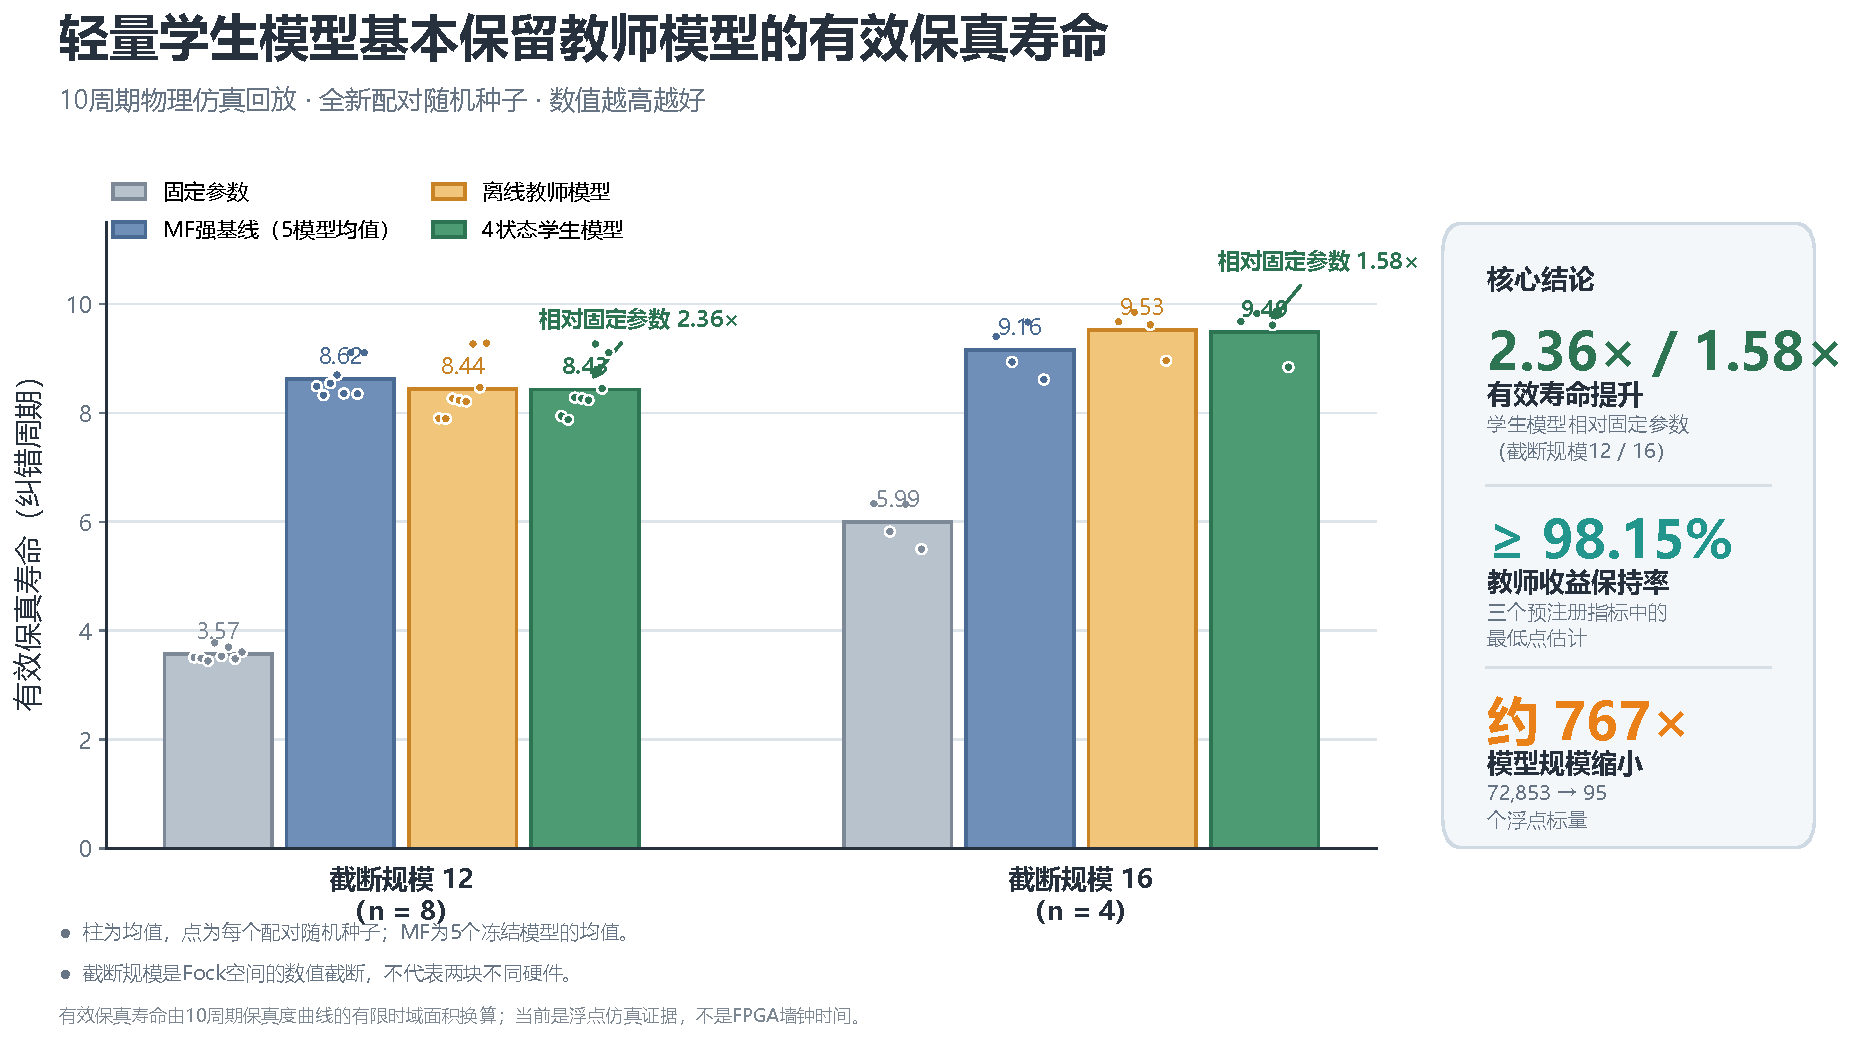
\includegraphics[width=\textwidth]{../figures/ppt_summary_20260716/effective_fidelity_lifetime_cn.pdf}
  \caption{Finite-model teacher--student extension evidence.  At cutoff 12
  ($n=8$ paired evaluation seeds), the four-state student reached an effective
  fidelity lifetime of 8.427 cycles versus 3.571 for fixed parameters, a
  $2.36\times$ ratio.  At cutoff 16 ($n=4$), the corresponding values were
  9.489 and 5.994 cycles, a $1.58\times$ ratio.  Bars show seed means and points
  show paired seeds; the MF bar is the mean of five frozen agents, not a
  test-selected winner.  The sidebar's 98.15\% is the lowest point retention,
  whereas the lowest paired-bootstrap 95\% interval lower bound is 94.45\%.
  All quantities are float finite-model results.}
  \label{fig:teacher-student-lifetime}
\end{figure}

The student closely tracked the offline teacher: their cutoff-12 lifetimes were
8.427 and 8.440 cycles, and their cutoff-16 lifetimes were 9.489 and 9.525
cycles.  The five-agent MF mean was slightly higher at cutoff 12 (8.623 cycles)
and lower at cutoff 16 (9.156 cycles), so the figure does not support universal
teacher superiority.  Across the three preregistered retention metrics, the
lowest student point retention was 0.981457 and the lowest 95\% interval lower
bound was 0.944501 relative to teacher-versus-standard gain.

The selected student uses four recurrent states and 95 stored scalars, versus
72,853 for the teacher, a $\sim767\times$ float-model compression.  Its
fixed-point RTL produced zero mismatches across 7,680 outputs, with maximum
fixed-versus-float error $1.46038\times10^{-4}$.

This is evidence for gain retention and compression within the project model.
It is not an official reproduction or improvement over Puviani \emph{et al.},
not a general memory-mechanism result, and not the main decoder LER claim.  The
larger quantized GRU lower-bound required 72,854 cycles (2,698.30 $\mu$s at
27 MHz), exceeded the five-microsecond slot, and was dropped.  That negative
result supports the architectural decision to keep learning outside the
critical fast path.

\section{Where the current data show an advantage}

Table~\ref{tab:advantage-matrix} is the compact answer to which metrics
currently show an advantage.  Rows are deliberately not collapsed into a
global score because decoder, controller, and hardware lanes have different
objects and units.

{\small
\begin{longtable}{@{}L{0.19\textwidth} L{0.18\textwidth} L{0.35\textwidth} L{0.18\textwidth}@{}}
\caption{Metric-level advantage matrix at the T6.7.2 evidence cutoff.}
\label{tab:advantage-matrix}\\
\toprule
Metric / property & Status & Evidence-supported statement & Boundary \\
\midrule
\endfirsthead
\toprule
Metric / property & Status & Evidence-supported statement & Boundary \\
\midrule
\endhead
Correlated-noise LER & \supported & Joint MAP error 0.23067 versus independent MAP 0.30883 in the strong-correlation paired Monte Carlo ($z=29.60$) & Ideal/model-level decoder evidence, not full \RouteA{} \\
Historical learned LER & \conditional & Hybrid Residual-B reduced T24 final LER by 1.75--2.89\% relative to UKF across four frozen scenarios & Old mock-backed software-HIL; not the new unified matrix \\
Smooth LER vs locked EWMA & \supported & \RouteA{} reduced aggregate LER by $2.1687\times10^{-5}$, 2.14\% relative, with a positive paired interval & Only the pre-registered EWMA contrast \\
Periodic-drift LER & \supported & Periodic EWMA-minus-\RouteA{} difference $8.618\times10^{-5}$; Holm-adjusted discovery & Effect does not generalize to the other three smooth families \\
LER vs static / Window & \blocked & \RouteA{} LER is higher than static and Window; oracle-gap closure is negative & Current evidence is counterevidence, not missing reporting \\
Smooth action balance & \conditional & 661 avoided versus 47 induced errors and zero false updates & High 21.6\% fallback signal; tied to smooth EWMA comparison \\
Abrupt/OOD vs locked EWMA & \conditional & All catastrophic, calibration-strict, and nominal non-inferiority gates passed & Five families are core-statistic ties; burst is aggregate-neutral; this is not a tail advantage \\
Tail LER vs static MAP & \blocked & Calibration worst was 181/512 for \RouteA{} versus 32/512 for static MAP & High tail fallback and false-update rates also remain visible \\
Fast-path determinism & \supported & Six-cycle arithmetic/action contract; million-cycle bit-exact qualification & Pre-board core/RTL evidence only \\
Target-device feasibility & \supported & Core and selected student exceed 39.5 MHz in three-seed post-route estimates and fit reported resources & Open-tool estimate; integrated \RouteA{} top and real board pending \\
Teacher--student finite-model extension & \supported & Effective fidelity lifetime was $2.36\times/1.58\times$ fixed parameters at cutoffs 12/16; retention point at least 0.981457; 95-scalar student with bit-exact RTL & Two-level, ten-cycle component/model evidence; not LER, wall-clock lifetime, or official GQF superiority \\
CNN as universal winner & \blocked & Learned strong branch failed; legacy CNN also violates new compute/state/workspace caps & CNN remains ablation or replaceable extension \\
Measured board speed / resources & \blocked & No real-board result is available & No fastest/SOTA or measured latency claim \\
\bottomrule
\end{longtable}
}

\section{Negative results that define the design}

The contract-centric narrative is credible only if its negative evidence is
kept visible.

\begin{enumerate}
  \item \textbf{The CNN-centric strong branch failed.}  The current main system
  cannot rely on a learned winner, and the historical CNN does not meet the new
  matched execution contract.
  \item \textbf{Static fallback and freeze-all adaptation failed.}  All 38
  candidate tuples were NO-GO for both V2 and V3 because a frozen trusted state
  became stale under persistent change.  Continuous validated shadows were an
  evidence-driven correction, not cosmetic refactoring.
  \item \textbf{Fallback is not free.}  The earlier uncertainty gate helped the
  aggregate OOD mixture but harmed compound OOD and slightly harmed nominal
  operation.  In the later formal matrix, registered non-inferiority passed,
  but tail fallback/unnecessary signals reached 59--96\% and 59--95\%.
  \item \textbf{The smooth primary gate is not a leaderboard.}  \RouteA{}
  passed the locked EWMA contrast but was worse than static and Window MAP, with
  negative oracle-gap closure and a gain concentrated in periodic drift.
  \item \textbf{Hardware evidence remains layered.}  CXXRTL, synthesis, P\&R,
  and a six-cycle contract do not imply a bitstream, transport integration,
  board timing, power, or quantum-device experiment.
\end{enumerate}

\section{Decisive remaining experiments}

The present note is intentionally a snapshot rather than a promotion decision.
The following gates determine how the final paper must be written.

\begin{table}[htbp]
\centering
\small
\caption{Remaining decision gates and mandatory downgrade paths.}
\label{tab:remaining-gates}
\begin{tabularx}{\textwidth}{@{}l X X@{}}
\toprule
Gate & Required evidence & Failure consequence \\
\midrule
T6.7.3 & At least $10^5$ cycles per family and $10^6$ aggregate integrated fixed-point/RTL cycles with zero action/state/reason/version mismatch & Keep deterministic core evidence only; no integrated-stack qualification \\
T6.7.4 & Independent recomputation of every LER, tail, nominal, and safety gate & Promote only the branches that pass; otherwise static MAP-LUT plus deterministic FPGA is the fallback paper \\
T6.8 & Same-trace static/drift comparison, official GQF reproduction, and task-normalized FPGA literature table & Claims remain internal-baseline and model-specific; no Puviani or FPGA superiority \\
T6.9 & Integrated top P\&R followed by real-board correctness, latency, deadline, resource, and power measurements & Hardware language remains estimate/qualification only \\
\bottomrule
\end{tabularx}
\end{table}

\section{Discussion}

The main contribution at this cutoff is a change in what is treated as the
scientific object.  A CNN-centric paper asks whether a particular learned
model wins.  The current system asks whether adaptation can be admitted,
audited, reverted, and compared under one causal execution contract.  This
change lets the project reuse the old affine parameter surface, frozen CNN
result, teacher/student work, fixed-point pipeline, and FPGA-oriented bank
machinery without allowing any one extension to carry unsupported system-wide
claims.

The smooth formal result illustrates both the value and the cost of this
framing.  Because EWMA was selected before formal access, the positive primary
interval is meaningful for that contrast.  Because static and Window were also
reported, the same experiment prevents a misleading best-method claim.  The
periodic family reveals a real routing opportunity, while the other smooth
families show that extra policy complexity can be neutral or harmful.  A
regime-aware method is therefore scientifically useful only if it says where
the regime logic helps and where it should stay out of the way.

The hardware line is similarly bounded.  Fixed cycles, packed words, atomic
banks, mutation-tested failures, P\&R estimates, and million-cycle bit parity
are stronger than a software-only latency sketch.  They are nevertheless one
layer below a measured control plane.  The eventual paper should report core,
transport, source-to-action, and end-to-end latency separately, and should
compare only with external work sharing a compatible task and timing
definition.

The tail matrix illustrates an important distinction between bounded safety and
performance advantage.  V4 passed every registered degradation margin against
locked EWMA, including nominal controls, so the policy did not reintroduce the
earlier compound failure.  Yet most contrasts are exact ties, static MAP is far
better under calibration shift, and safety signals are active through much of
the tail interval.  The honest interpretation is auditable locked-baseline
non-inferiority with high intervention cost.  Whether the integrated integer
router preserves even that bounded statement remains subject to T6.7.3 and the
independent T6.7.4 promotion/falsification audit.

\section{Conclusion}

The current evidence supports a contract-centric, regime-aware dual-loop
architecture as a disciplined way to separate GKP decoding performance,
tail-safety control, and deterministic execution.  Quantitatively, \RouteA{}
has a positive untouched smooth contrast against the pilot-locked EWMA
baseline and a Holm-corrected periodic-drift advantage.  The same data show
that static and Window MAP remain better in aggregate, so general LER
superiority is not established.  Abrupt/OOD evidence supports registered
non-inferiority to locked EWMA, not tail or static-MAP superiority.
Hardware-facing evidence supports a
six-cycle fixed-point contract, target-device feasibility, and million-cycle
board-independent bit parity, but not measured FPGA speed or external
leadership.  Historical CNN and teacher/student results remain valuable as
replaceable extension evidence rather than as the identity of the system.

This evidence partition is the central result of the current note.  It makes
the eventual claim contingent on integrated-RTL, independent promotion,
external, and real-board gates, and it preserves explicit downgrade paths if
those gates fail.

\appendix

\section{Primary repository evidence map}

\begin{longtable}{@{}p{0.19\textwidth} p{0.35\textwidth} p{0.36\textwidth}@{}}
\toprule
Topic & Human-readable source & Machine/source-data source \\
\midrule
\endfirsthead
\toprule
Topic & Human-readable source & Machine/source-data source \\
\midrule
\endhead
Claim and role contract & \path{docs/route_a_claim_contract.md} & \path{docs/t6_5_1_route_a_claim_contract.json} and CSV \\
Unified execution contract & \path{docs/unified_execution_contract.md} & \path{docs/t6_5_2_unified_execution_contract.json} and CSV \\
Formal preregistration & \path{docs/route_a_preregistration.md} & \path{docs/t6_5_3_route_a_preregistration.json} and CSV \\
Comparator qualification & \path{docs/unified_comparator_runner.md} & \path{docs/t6_6_1_unified_comparator_runner.json} and CSV \\
V4 policy & \path{docs/regime_aware_safe_policy.md} & \path{docs/t6_6_2_regime_aware_safe_policy.json} and CSV \\
Posterior/threshold lock & \path{docs/route_a_posterior_calibration.md} & \path{docs/t6_6_3_route_a_posterior_threshold_lock.json} and CSV \\
Smooth formal matrix & \path{docs/route_a_smooth_formal.md} & \path{docs/t6_7_1_smooth_formal_matrix.json} and 498,240-row CSV \\
Abrupt/OOD formal matrix & \path{docs/route_a_tail_formal.md} & \path{docs/t6_7_2_abrupt_ood_tail_formal_matrix.json} and 686,104-row CSV \\
Legacy frozen result & \path{docs/paper_materials/paper_simulation_result_table_pack.md} & \path{runs/p4_benchmark/T24_formal_software_revalidation_20260510_200743/comparison.csv} \\
Target P\&R & \path{docs/target_device_synthesis.md} & \path{docs/t5_5_2_target_device_synthesis.json} and raw reports \\
Student Pareto & \path{docs/precision_resource_performance_pareto.md} & \path{docs/t5_5_3_precision_resource_pareto.json} and equivalence report \\
Long RTL qualification & \path{docs/long_rtl_qualification.md} & \path{docs/t6_2_2_long_rtl_qualification.json} and CSV \\
Dual-loop presentation schematic & \path{docs/figures/ppt_summary_20260716/drift_adaptive_architecture_cn.pdf} & \path{docs/figures/make_ppt_summary_figures.py} \\
Teacher--student presentation figure & \path{docs/figures/ppt_summary_20260716/effective_fidelity_lifetime_cn.pdf} & \path{docs/t4_4_4_teacher_student_gain_retention_source_data.csv} and figure generator \\
\bottomrule
\end{longtable}

\section{Claim wording guardrails}

\begin{itemize}
  \item Allowed now: ``improves over the pilot-locked EWMA baseline on the
  untouched smooth aggregate, with the family-level discovery concentrated in
  periodic drift.''
  \item Allowed now: ``passed the pre-registered abrupt/OOD and nominal
  non-inferiority gates relative to locked EWMA; most core contrasts were
  ties.''
  \item Not allowed now: ``outperforms static GKP decoding'', ``best adaptive
  decoder'', ``improves tail LER'', ``outperforms under OOD'', or ``CNN
  provides the main gain.''
  \item Allowed now: ``the fixed-point core has a six-cycle contract and passed
  board-independent CXXRTL and target-device P\&R qualification.''
  \item Not allowed now: ``measured sub-microsecond FPGA decoder'', ``faster
  than existing FPGA QEC decoders'', or ``hardware validated.''
  \item Allowed now: ``the distilled student retained most teacher gain in the
  project finite model and fit a selected pre-board design point.''
  \item Not allowed now: ``reproduces or exceeds Puviani NMF'' or ``proves a
  universal non-Markovian memory advantage.''
\end{itemize}

\begin{thebibliography}{9}

\bibitem{gkp2001}
D. Gottesman, A. Kitaev, and J. Preskill,
``Encoding a qubit in an oscillator,''
\emph{Physical Review A} \textbf{64}, 012310 (2001).

\bibitem{grimsmo2021}
A. L. Grimsmo and S. Puri,
``Quantum error correction with the Gottesman--Kitaev--Preskill code,''
\emph{PRX Quantum} \textbf{2}, 020101 (2021).

\bibitem{chen2022}
E. H. Chen \emph{et al.},
``Calibrated decoders for experimental quantum error correction,''
\emph{Physical Review Letters} (2022).

\bibitem{sivak2024}
V. Sivak, M. Newman, and P. Klimov,
``Optimization of decoder priors for accurate quantum error correction,''
\emph{Physical Review Letters} \textbf{133}, 150603 (2024).

\bibitem{puviani2025}
M. Puviani, S. Borah, R. Zen, J. Olle, and F. Marquardt,
``Non-Markovian feedback for optimized quantum error correction,''
\emph{Physical Review Letters} \textbf{134}, 020601 (2025).

\bibitem{sivak2023}
V. Sivak \emph{et al.},
``Real-time quantum error correction beyond break-even,''
\emph{Nature} (2023).

\end{thebibliography}

\end{document}
